\newpage
{\color{gray}\hrule}
\begin{center}
\section{Rivelazione della radiazione $\beta^{-}$}
\bigskip
\end{center}
{\color{gray}\hrule}    
Per la seconda parte dell'esperienza, volta alla rivelazione della radiazione $\beta^{-}$, si utilizza un Supporto SP5608 con lastra di scintillatore in polistirene (area attiva: 4.7x4.7x1 cm$^3$) avvolta in nastro di teflon e un SiPM a 14400 celle in 6.0x6.0mm$^2$; l'utilizzo di un SiPM con più celle rispetto a quello della prima parte permette di avere misure più precise, a discapito di un aumento del DCR e di una maggiore probabilità di OCT.
Inoltre, come prima, l’unità di alimentazione e amplificazione (PSAU) fornisce segnali analogici in tensione, ricevuti e convertiti in canali dal Digitizer.

La radiazione di tipo $\beta^{-}$ ha origine dal decadimento di un neutrone $n$ in un protone $p$ con l'emissione di un elettrone $e^-$ e un anti-neutrino elettronico $\bar \nu_e$, $$n \rightarrow p + e^- + \bar \nu_e$$
L’elettrone emesso ($\beta^-$) può incidere sullo scintillatore, interagire con gli elettroni legati agli atomi del materiale plastico e cedere tutta la sua energia cinetica iniziale. L'energia trasferita eccita gli atomi a livelli superiori, i quali, diseccitandosi, ritornano allo stato fondamentale emettendo fotoni nel visibile (tipicamente $\lambda \approx 425$ nm). Solo una parte ($\sim30\%$) della luce di scintillazione viene rivelata dal SiPM e convertita in un segnale elettrico proporzionale al flusso di fotoni. \\ Una volta calibrato in energia lo spettro, sarà possibile caratterizzare la radiazione $\beta^-$ emessa dalle sorgenti di $^{90}\mathrm{Sr}$ e $^{137}\mathrm{Cs}$. \\
Infine, verrà analizzata la capacità di assorbimento della radiazione $\beta^-$ di due diversi materiali, alluminio e carta, con lo scopo di ricavare alcune caratteristiche di questi ultimi. \\

\subsection{Spettro ${}^{90}$Sr}
Il decadimento di ${}^{90}$Sr produce Ittrio-90 e avviene tramite emissione $\beta^-$ durante la reazione
$$^{90}\mathrm{Sr} \rightarrow {}^{90}\mathrm{Y} + e^- + \bar{\nu}_e $$
A sua volta, anche $^{90}\mathrm{Y}$ decade in Zirconio-90 tramite emissione $\beta^-$, seguendo $$^{90}\mathrm{Y} \rightarrow {}^{90}\mathrm{Zr} + e^- + \bar{\nu}_e $$
\textit{Osservazione.} Si anticipa che il tempo di dimezzamento dell'Ittrio-90 è tanto piccolo rispetto a quello dello Stronzio-90 da non permettere di isolare i due spettri, che risulteranno quindi sovrapposti.
\subsubsection{Fattore di calibrazione $k_{Sr}$ dell'apparato con sorgente in asse}
Una volta posizionata la sorgente in asse con il fotomoltiplicatore, si acquisisce dal Digitizer uno spettro costituito da circa 2 milioni di eventi. Durante l’intera fase di presa dati è fondamentale mantenere il sistema quanto più possibile isolato dalla luce esterna, così da minimizzare il rumore; inoltre, si utilizza come \textit{trigger} esterno il segnale proveniente dallo stesso SiPM, impostando una soglia di discriminazione $V_{thr}$\footnote{Per tutta questa sezione si è impostato $V_{thr} = -6$ mV} in corrispondenza del punto in cui termina l'andamento esponenziale del \textit{rate} visualizzabile sullo Staircase plot.

\textit{Osservazione.} Il rivelatore SiPM+scintillatore è adatto per spettroscopia $\beta^-$ in quanto le particelle provenienti dalla sorgente si fermano nel polistirene cedendo tutta la loro energia cinetica iniziale. Lo spettro in energia che si ottiene è approssimabile all'energia degli elettroni acquisita nella reazione di decadimento. Quest'ultima inoltre non è monocromatica ma varia in modo continuo da 0 ad un valore massimo $T_{max}$. 

Si riporta di seguito lo spettro in energia di ${}^{90}$Sr con sorgente in asse.
\begin{figure} [H]
    \centering
    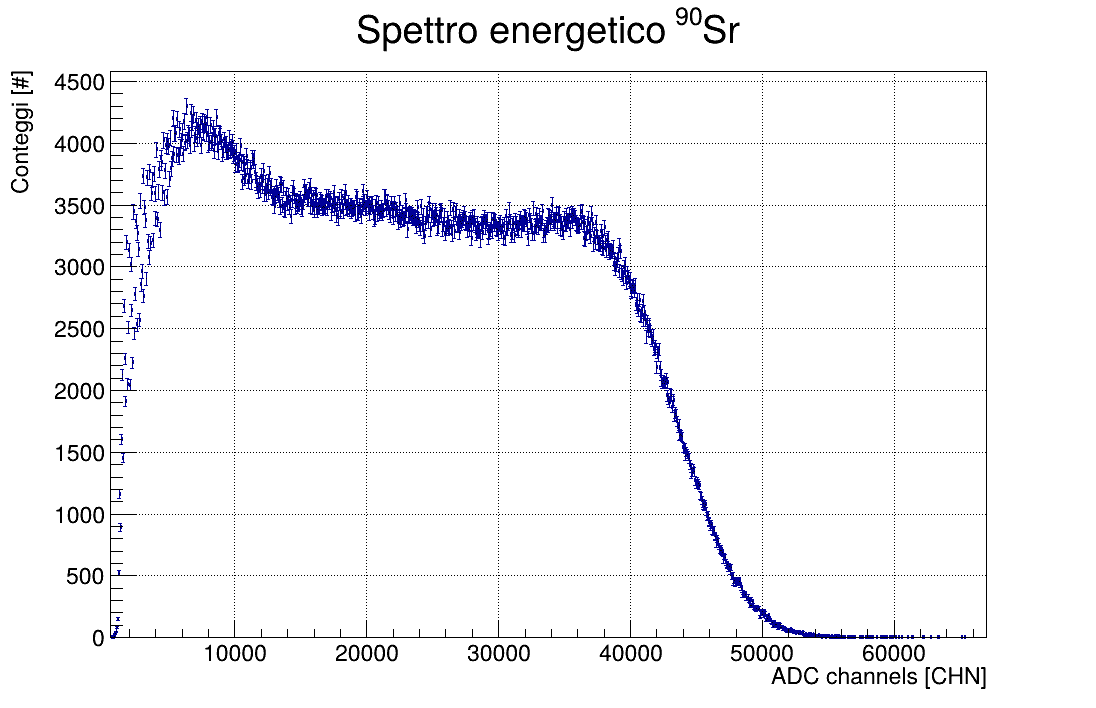
\includegraphics[width=0.65\linewidth]{fig2/sr90_tot.png}
    \caption{ \footnotesize Istogramma di conteggi per numero di canale dello ${}^{90}$Sr}
    \label{fig:Sr90_tot}
\end{figure}

L'istogramma mostra la sovrapposizione dei due spettri: in particolare si osserva un contributo a energie più basse associato a ${}^{90}\mathrm{Sr}$, mentre ${}^{90}\mathrm{Y}$, 
caratterizzato da un’\textit{end-point} $T_{0,Y}$ maggiore, domina la regione a energie più elevate, determinando l’estensione complessiva dello spettro.\\
La sovrapposizione degli spettri impedisce di riconoscere il $T_{0,Sr}$ dello Stronzio-90, mentre è possibile misurarne il $T_{max, Sr}$; viceversa, per l'Ittrio-90 non è individuabile il $T_{max, Y}$, mentre è possibile misurarne il $T_{0, Y}$.

Dalla misura sperimentale dell'\textit{end-point} $CHN_{0,Y}$ dell'Ittrio-90 è possibile ricavare la costante di calibrazione $k_{Sr}$ del sistema mediante la formula 
\begin{equation}
    k_{Sr}=\frac{T_{0,Y}}{CHN_{0,Y}}
    \label{eq:k}
\end{equation} dove in letteratura l'\textit{endpoint} dello Ittrio-90 è $T_{0,Y}= (2.28\pm 0.04)$ MeV.\\
Per ottenere una stima di $CHN_{0,Y}$, nella regione di \textit{end-point} si effettua un plot di Kurie, consistente in una regressione lineare sulle coppie di dati ($\frac{\sqrt{conteggi}}{CHN}$,$CHN$), riportata di seguito nel grafico \ref{fig:kurie_cen}.

\begin{figure} [H]
    \centering
    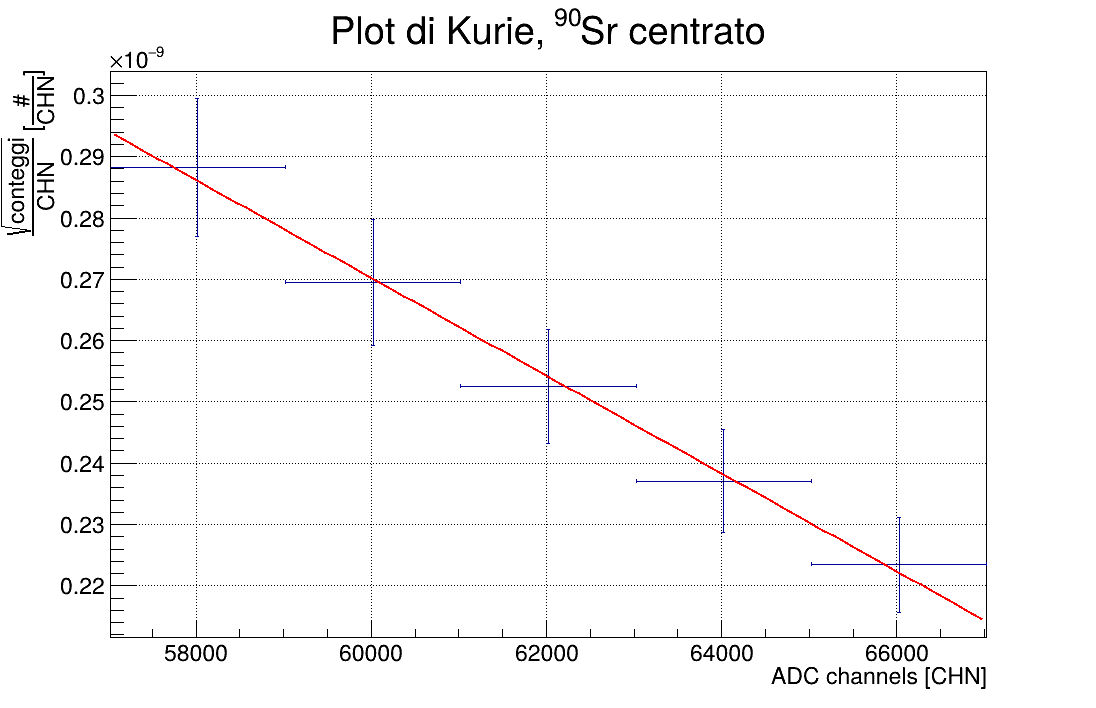
\includegraphics[width=0.65\linewidth]{fig2/kurie_cen.png}
    \caption{ \footnotesize Istogramma ($CHN$,$\frac{\sqrt{conteggi}}{CHN}$) e regressione lineare $y=a+bx$ con parametri restituiti $a = ( 7.5 \pm 0.9 )\cdot 10^{-10} \text{ CHN }^{-1}$, $b= (-8.0\pm1.5)\cdot 10^{-15} \text{CHN}^{-2}$, $\chi^2=0.11$ e d.o.f.$=3$}
    \label{fig:kurie_cen}
\end{figure}

Dal fit si estrapola $CHN_{0,Y}= ( 9 \pm 2 )\cdot10^4 \text{ CHN}$

Infine, si calcola il fattore di calibrazione $k_{Sr}$ dell'apparato con sorgente in asse dalla \ref{eq:k}:
\begin{equation}
    k_{Sr}=( 2.4 \pm 0.5 )\cdot10^{-5} \text{ MeV/CHN }
    \label{eq:k_Sr}
\end{equation}
Con questa stima è possibile convertire in energia ogni valore espresso in CHN: $E=k\cdot CHN$.
\subsubsection{Verifica sperimentale di $T_{max,Sr}$}
In questa sezione, si verifica sperimentalmente che la stima del valore di energia più probabile $T_{max, Sr}$, ottenuta tramite un fit parabolico (vedi figura \ref{fig:sr90_max}) nella regione corrispondente al picco, è compatibile con il valore atteso per lo spettro dello Stronzio-90, $T_{max,Sr, att} \approx 0.38\cdot T_{0,Sr}$, dove in letteratura $T_{0,Sr}=0.546$ MeV.
\begin{figure} [H]
    \centering
    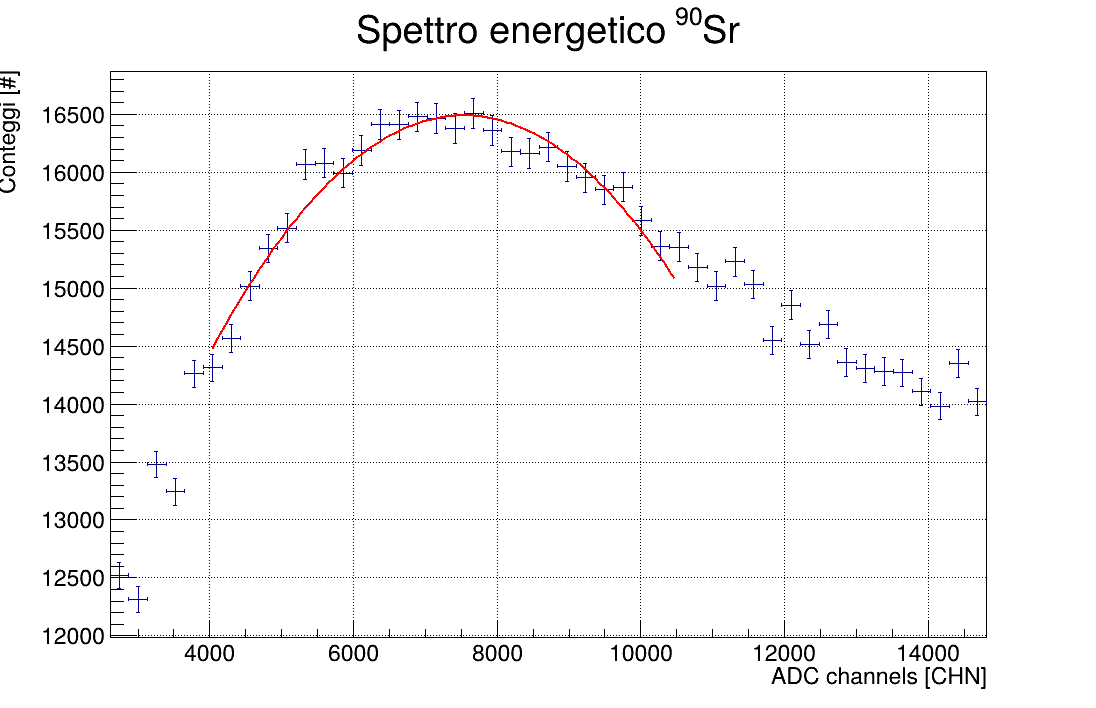
\includegraphics[width=0.64\linewidth]{fig2/sr90_max.png}
    \caption{ \footnotesize Istogramma di conteggi per numero di canali del ${}^{90}$Sr (con accorpamento di \textit{bin}) e fit parabolico $y=ax^2+bx+c$ con parametri restituiti
    $a= ( -1.64 \pm 0.08 )\cdot10^{-4} \text{ CHN }^{-2}$,
    $b= ( 2.47 \pm 0.11 ) \text{ CHN }^{-1}$,
    $c= 7200 \pm 400 $,
    , $\chi^2=30$ e d.o.f.$=22$}
    \label{fig:sr90_max}
\end{figure}
Prima si è estratta dal fit parabolico la stima del picco $CHN_{max, Sr}=( 7.5 \pm 0.5 )\cdot10^3 \text{ CHN }$ che è stata poi convertita in energia: $$T_{max, Sr}= ( 0.18 \pm 0.04 ) \text{ MeV }$$
che è statisticamente compatibile con il valore atteso.

\subsubsection{Fattore di calibrazione $k_{Sr,eq}$ dell'apparato con sorgente fuori asse}
Si ripete l’acquisizione dello spettro di ${}^{90}$Sr posizionando la sorgente in una configurazione fuori asse, ovvero a una distanza $r_{eq}$ dal centro dello scintillatore. \\Si può dimostrare infatti che il fattore di calibrazione medio $k_\text{Sr,eq}$, nel caso in cui i segnali colpiscano con uguale probabilità qualsiasi punto della lastra, è equivalente a quello ottenuto per una sorgente puntiforme posta a una distanza $r_{eq} = 0.3826 \cdot l$ dal centro, dove $l$ rappresenta il lato dello 
scintillatore quadrato. \\
Tale scelta consente quindi di stimare il nuovo fattore di calibrazione $k_{Sr,eq}$, utile successivamente per le misure dei raggi cosmici, poiché gli eventi non provengono da una sorgente puntiforme, ma da tutte le direzioni.\\
Dunque, analogamente a quanto fatto nel paragrafo 2.2.1, si procede all’analisi dei dati con il plot di Kurie (vedi grafico \ref{fig:kurie_decen}). 
\begin{figure} [H]
    \centering
    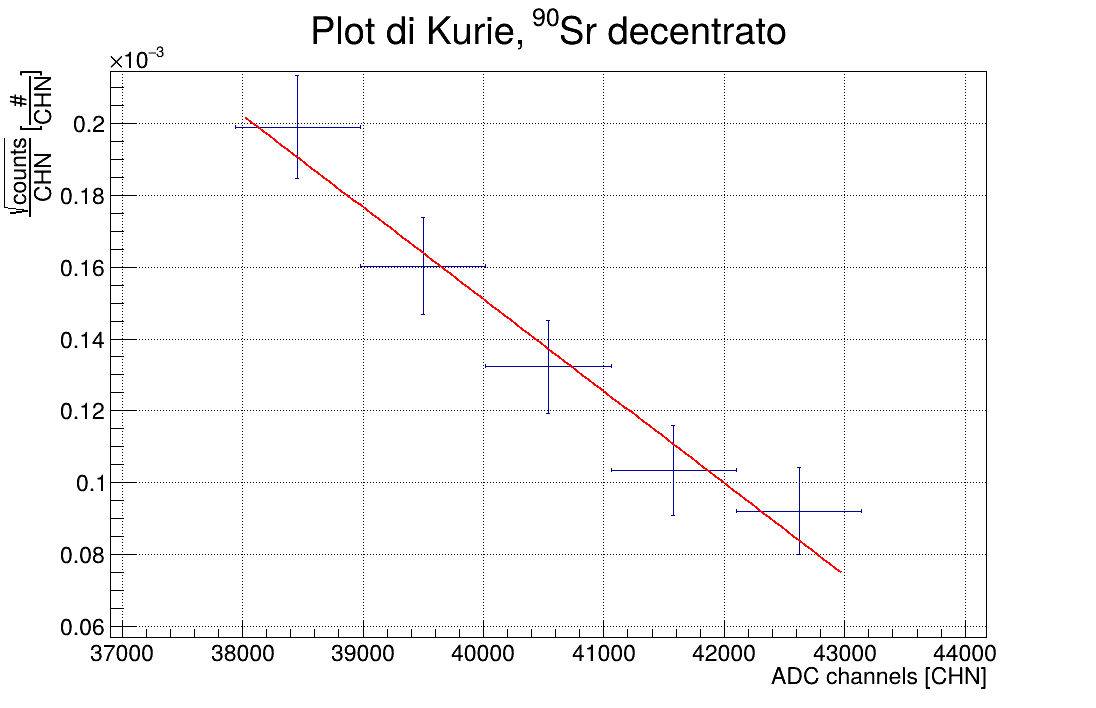
\includegraphics[width=0.7\linewidth]{fig2/kurie_decen.png}
    \caption{ \footnotesize Istogramma ($CHN$,$\frac{\sqrt{conteggi}}{CHN}$) e regressione lineare $y=a+bx$ con parametri restituiti $a= ( 1.18 \pm 0.16 )\cdot10^{-3}\text{ CHN }^{-1}$, $b= ( -2.6 \pm 0.4 )\cdot10^{-8} \text{ CHN }^{-2}$, $\chi^2=1.4$ e d.o.f.$=3$}
    \label{fig:kurie_decen}
\end{figure}

Come prima, dal fit si estrapola $CHN_{0,Y}= ( 4.6 \pm 1.0 )\cdot10^4 \text{ CHN}$ e si ricava infine il nuovo fattore di calibrazione $k_{Sr,eq}$ dell'apparato con sorgente fuori asse dalla formula \ref{eq:k}:
$$k_{Sr,eq}=( 5.0 \pm 1.0 )\cdot10^{-5} \text{ MeV/CHN }$$
Con $k_{Sr,eq}$ è possibile convertire in energia i valori espressi in CHN: $E=k_{Sr,eq}\cdot CHN$. \\

\subsection{Assorbimento della radiazione $\beta^{-}$ nei materiali} 
Tra la sorgente ${}^{90}$Sr e il rivelatore si inseriscono in modo crescente da 1 a 20 foglietti di carta o alluminio e, a gruppi di 2 o 3, se ne misurano i corrispondenti \textit{rate}, effettuando anche anche una misura senza foglietti.

Segue l'analisi per entrambi i materiali.

\subsubsection{Assorbimento con carta}
Tramite un calibro (sensibilità $0.05$mm) si misura lo spessore di un foglietto di carta $d_{carta}$ a partire dallo spessore totale dei 20 foglietti. $$d_{carta} = ( 0.100 \pm 0.003 ) \text{ mm} $$ 
Per ogni istogramma dei conteggi per numero di impulsi ricevuti associato all'aggiunta dei foglietti, si estraggono\footnote{Come per il \textit{dark count rate}, si è impostato un \textit{gate} di 500ms e si è riconvertita la stima in Hz.} media $\nu_i$ e deviazione standard $\sigma_{\nu,i}$, riportati in tabella \ref{tab:carta}. Tutti gli istogrammi sono riportati in appendice 5.3.1.

Si grafica il \textit{rate} $\nu $ in funzione dello spessore e si effettua sui dati un fit esponenziale per verificare legge di assorbimento dei raggi $\beta^-$: 
\begin{equation}
    N(x) = N(0)e^{-\mu x}
    \label{eq:assorb}
\end{equation}
dove N è il numero di particelle trasmesse dal materiale, $x$ spessore del materiale e $\mu$ coefficiente di assorbimento.\\
\begin{multicols}{2}
    \begin{figure} [H]
    \centering
    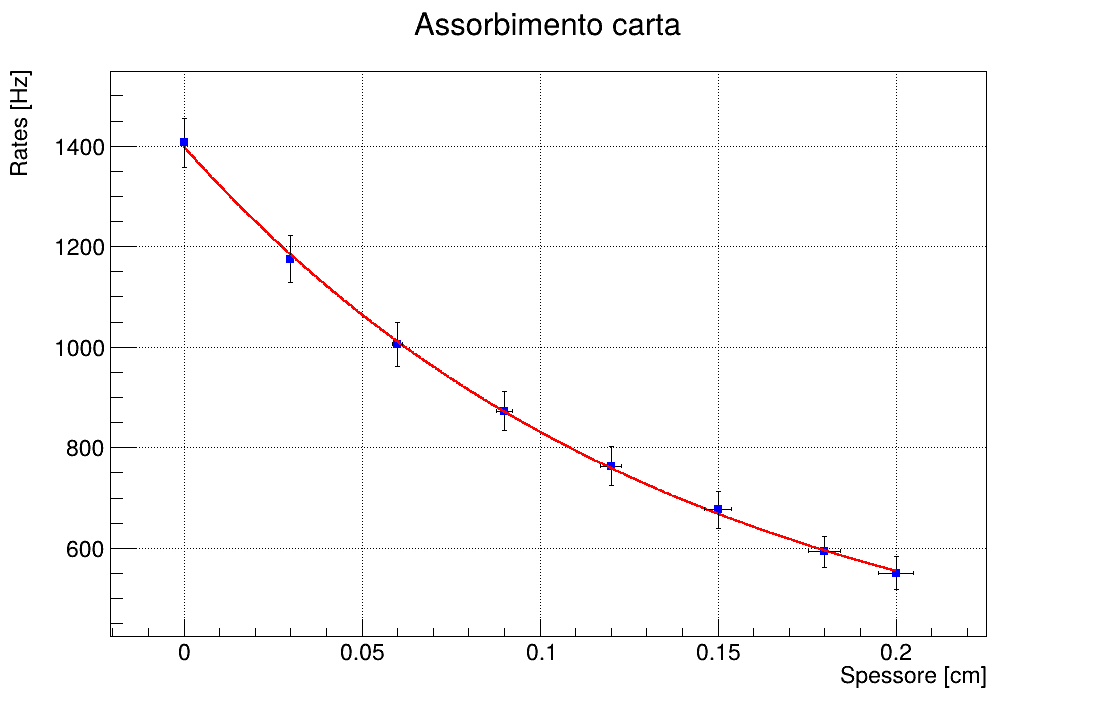
\includegraphics[width= \linewidth]{fig2/ass_carta.png}
    \caption{ \footnotesize Coppie di dati ($x$,$\nu$) e fit esponenziale \\ $y=a+be^{-cx}$ con parametri restituiti $a= ( 2.9 \pm 1.5 ) \text{$10^{2}$ Hz}$, $b= ( 11.1 \pm 1.3 ) \text{ $10^{2}$ Hz}$, $c= ( 7 \pm 2 ) \text{cm$^{-1}$ }$ e $\chi^2=0.15$ e d.o.f.=$5$}
    %\label{fig:2.3}
\end{figure}
\begin{table}[H]
    \centering
    \begin{tabular}{|c|c|c|c|}
        \hline
        
        \textbf{$n$[$\#$]} & \textbf{$x$[mm]} & \textbf{$(\nu \pm \sigma_\nu )$[$10^{2}$ Hz]} \\ \hline
        
        $ 0$  &  $ 0.000  \pm  0.003 $  &  $ 14.1 \pm  0.5 $   \\ \hline
        $ 3 $  &  $ 0.300  \pm  0.008 $  &  $ 11.8  \pm  0.5 $   \\ \hline
        $ 6 $  &  $ 0.600  \pm  0.015 $  &  $ 10.1  \pm  0.4 $  \\ \hline
        $ 9 $  &  $ 0.90  \pm  0.02 $  &  $ 8.7  \pm  0.4 $   \\ \hline
        $ 12 $  &  $ 1.20  \pm  0.03 $  &  $ 7.6  \pm  0.4 $  \\ \hline
        $ 15 $  &  $ 1.50  \pm  0.04 $  &  $ 6.8  \pm  0.4 $   \\ \hline
        $ 18 $  &  $ 1.80  \pm  0.05 $  &  $ 6.0  \pm  0.3 $  \\ \hline
        $ 20 $  &  $ 2.00  \pm  0.05 $  &  $ 5.5  \pm  0.3 $   \\ \hline
        
    \end{tabular}
    \caption{\footnotesize Valori di numero di foglietti $n$, spessore di materiale attraversato $x$, media $\nu$ e rispettiva deviazione std $\sigma_{\nu}$ alla tensione $V_{bias}=54$V e \textit{gain} $G_{ampl}=28$dB.}
    \label{tab:carta}    
\end{table}

\end{multicols}

Il parametro $c$ estratto dal fit fornisce una stima del coefficiente di assorbimento $$\mu_{carta} = ( 7\pm 2 ) \text{ cm$^{-1}$}$$ Il valore ottenuto è comparabile quello atteso atteso per elettroni con \textit{end point} di 2.2MeV nella carta:
$\mu_{carta,att}\in [ 3.5,6.5]\text{cm}^{-1}$. 

\textit{Osservazione.} Dalla visualizzazione dello spettro energetico di ${}^{90}$Sr con un numero crescente di foglietti di carta si osserva che la parte dello spettro più affetta dall'assorbimento del materiale è quella in corrispondenza di basse energie; le particelle incidenti con energia minore vengono infatti assorbite prima di raggiungere il rivelatore.

\subsubsection{Assorbimento con alluminio}
Al contrario, per l'alluminio si può calcolare lo spessore di un singolo foglietto $d_{Al}$ conoscendo il suo coefficiente di assorbimento $\mu_{Al}=(14.5 \pm 0.5) \text{cm}^{-1}$. \\
Per ogni istogramma dei conteggi per numero di impulsi ricevuti associato all'aggiunta dei foglietti, si estraggono\footnote{Come per la carta, si è impostato un \textit{gate} di 500ms e si è riconvertita la stima in Hz.} media $\nu_i$ e deviazione standard $\sigma_{\nu,i}$, riportati in tabella \ref{tab:all}. Tutti gli istogrammi sono riportati in appendice 5.3.2.\\
Si grafica il rate in funzione del numero di foglietti e si effettua sui dati un fit esponenziale per verificare legge \ref{eq:assorb} di assorbimento dei raggi $\beta^-$.\\

\begin{multicols}{2}
\begin{figure} [H]
    \centering
    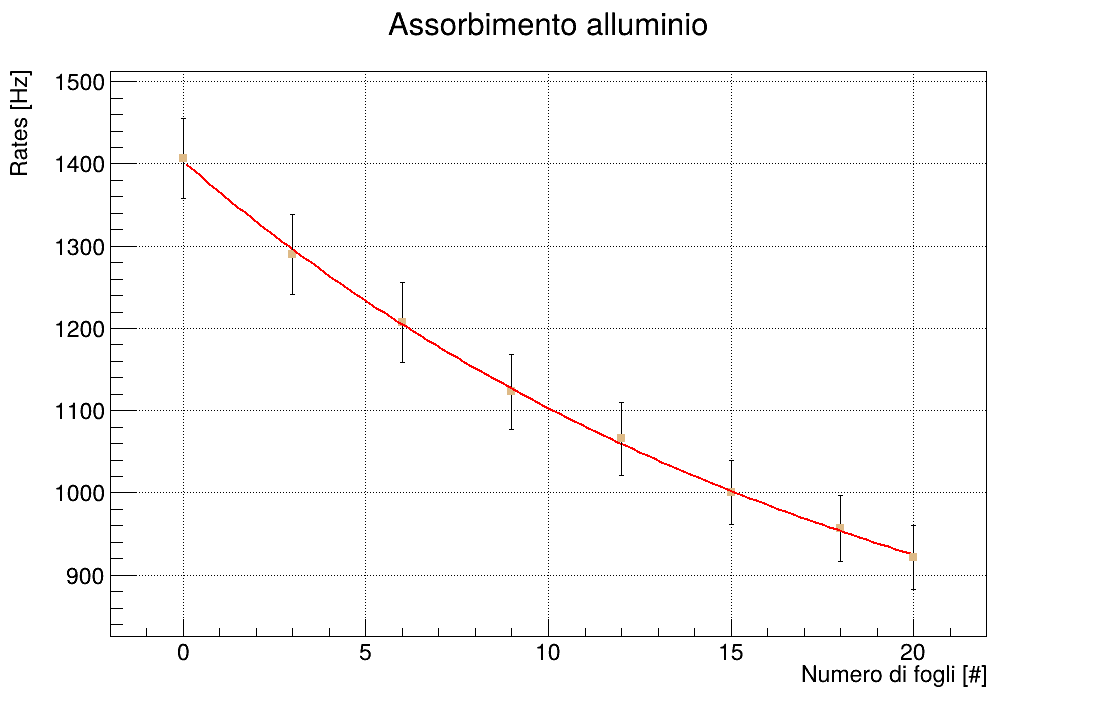
\includegraphics[width=1.\linewidth]{fig2/ass_all.png}
    \caption{ \footnotesize Coppie di dati ($n$,$\nu$) e fit esponenziale \\ $\nu=a+be^{-cn}$ con parametri restituiti $a= ( 0.7\pm 0.3 ) \text{kHz}$, $b= ( 0.7 \pm 0.3 ) \text{ kHz}$, $c= ( 0.05 \pm 0.04 ) \text{}$ e $\chi^2=0.07$ e d.o.f.=$5$}
   % \label{fig:2.3}
\end{figure}

\begin{table}[H]
    \centering
    \begin{tabular}{|c|c|c|}
        \hline
        
        \textbf{$n$[$\#$]} & \textbf{$(\nu \pm \sigma_\nu )$[$10^{2}$Hz]}  \\ \hline
        $ 0 $  &  $ 14.1  \pm  0.5 $  \\ \hline        
        $ 3 $  &  $ 12.9  \pm  0.5 $  \\ \hline
        $ 6 $  &  $ 12.1  \pm  0.5 $   \\ \hline
        $ 9 $  &  $ 11.2  \pm  0.5 $  \\ \hline
        $ 12 $  &  $ 11.0  \pm  0.4 $   \\ \hline
        $ 15 $  &  $ 10.0  \pm  0.4 $  \\ \hline
        $ 18 $  &  $ 9.6  \pm  0.4 $ \\ \hline
        $ 20 $  &  $ 9.2  \pm  0.4 $  \\ \hline
        
    \end{tabular}
    \caption{\footnotesize Valori di numero di foglietti $n$, media $\nu$ e deviazione std $\sigma_{\nu}$ alla tensione $V_{bias}=54$V e \textit{gain} $G_{ampl}=28$dB.}
    \label{tab:all}    
\end{table}
\end{multicols}

Questa volta, dal fit si estrae il prodotto $c=\mu_{Al}d_{Al}$, allora la stima dello spessore di un singolo foglietto di alluminio usando il valore teorico di $\mu_{Al}$ è $$d_{Al}= ( 0.04 \pm 0.03 ) \text{ mm}$$

Come per la carta, all'aumentare del numero di foglietti di alluminio la parte di spettro che subisce un maggior assorbimento è quella in corrispondenza delle basse energie.
\newpage
\subsection{Spettro ${}^{137}\text{Cs}$}
Nel $94.6\%$ dei casi il decadimento del Cesio-137 in Bario-137 avviene tramite emissione $\beta^-$ seguendo la reazione $$^{137}\mathrm{Cs} \rightarrow {}^{137}\mathrm{Ba(^*)} + e^- + \bar{\nu}_e $$
dove $^{137}\mathrm{Ba(^*)}$ è una forma instabile del Bario-137, la quale a sua volta può diseccitarsi emettendo un $\gamma$ con una probabilità dell'85.1$\%$:
$$^{137}\mathrm{Ba(^*)} \rightarrow {}^{137}\mathrm{Ba} + \gamma$$
Poiché la sorgente non è infinitamene sottile, la radiazione $\gamma$ emessa può estrarre per effetto fotoelettrico radiazione $\beta^-$ monocromatica:
\begin{equation}
    E_e = E_{\gamma} - B_e
    \label{eq:gamma}
\end{equation}
Tale fenomeno prende il nome di conversione interna; inoltre il $\beta^-$ estratto da $\gamma$ può appartenere a due K-shell diverse, rispettivamente a più bassa e a più alta energia di legame (624 keV e \\ 656 keV).

In alternativa, il Cesio-137 può decadere nel $5.4\%$ dei casi già nel livello stabile del Bario-137 
$$^{137}\mathrm{Cs} \rightarrow {}^{137}\mathrm{Ba} + e^- + \bar{\nu}_e $$


\subsubsection{Misura del picco di conversione interna $E_{ci}$}
Si acquisisce lo spettro completo in energia del ${}^{137}$Cs, riportato nella figura \ref{fig:cesio}, per la misura del picco di conversione interna $E_{ci}$.

\begin{figure} [H]
    \centering
    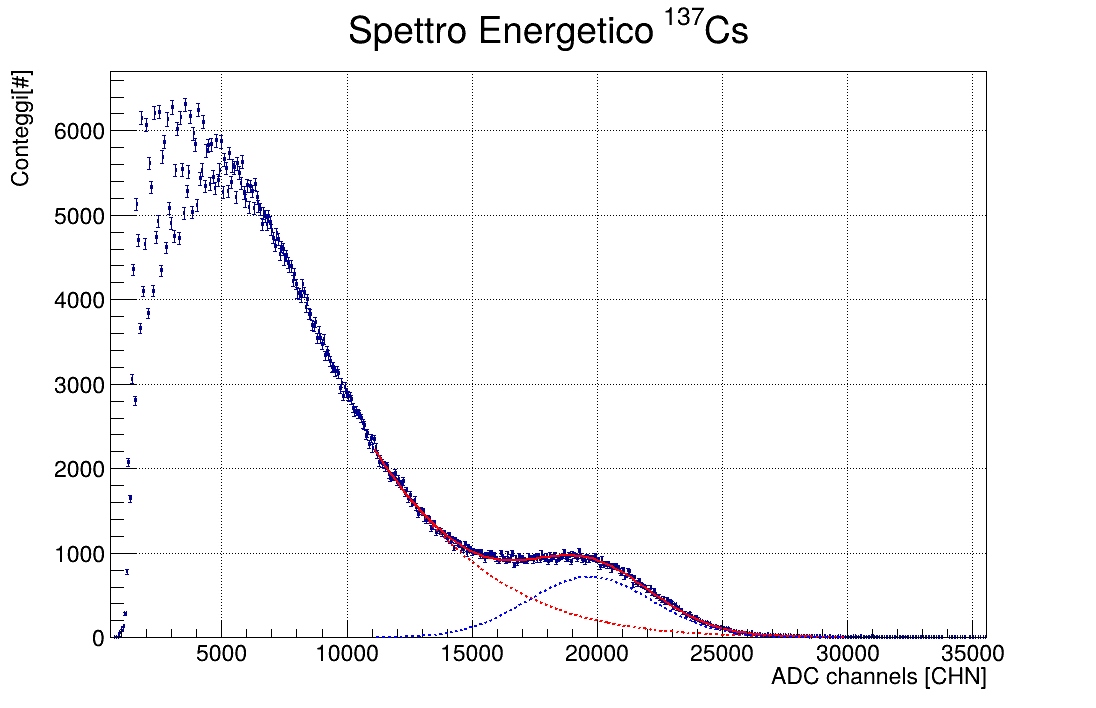
\includegraphics[width=0.75\linewidth]{fig2/cs137_conv_int.png}
    \caption{ \footnotesize Istogramma di conteggi per numero di canale del ${}^{137}$Cs, con fit di due gaussiane sovrapposte, $\chi^2=325$ e d.o.f$=286$. Sono state rappresentate le due gaussiane sommate con linee tratteggiate.}
    \label{fig:cesio}
\end{figure}

Dal grafico si può osservare l'effetto della conversione interna in corrispondenza del  secondo picco. Questo è in realtà generato dalla sovrapposizione dei due picchi relativi alle due K-shell diverse, ma la capacità risolutiva dello strumento non permette di distinguerli.

Si effettua allora un fit combinato della coda destra di una gaussiana per modellare l'andamento decrescente e di una gaussiana nella zona del picco di conversione interna. I parametri con le relative incertezze del fit sono riportate in appendice 5.2.4.

Si estraggono dal fit la posizione del picco dal valore medio della gaussiana $\langle CHN\rangle_{ci}$ e la sua deviazione standard $\sigma_{\langle CHN\rangle}$
$$\langle CHN\rangle_{ci} = ( 20 \pm 3 )\cdot10^3 \text{ CHN }$$ Convertendo in energia tramite la stima del fattore di calibrazione dello Stronzio-90 $k_{Sr}$ (\ref{eq:k_Sr}) si ottiene il valore sperimentale del picco di conversione interna $$\langle E\rangle_{ci} = ( 470 \pm 120 ) \text{ keV }$$
È stata infine verificata la compatibilità statistica tra la stima sperimentale $\langle E\rangle_{ci}$ e il valore teorico $E_{ci,att}$, ottenuto dalla media pesata\footnote{Con peso 4 per il picco teorico a $624$keV e peso 1 per quello a $656$keV} tra le energie dei due picchi:
$$E_{ci,att} = ( 629 \pm 16 ) \text{ keV }$$
Da questi parametri si stima anche la risoluzione sperimentale
\begin{equation}
R_\text{exp} = \frac{\sigma_{\langle CHN\rangle}}{\langle CHN_{ci}\rangle} = 0.128\pm0.016
\label{eq:R_exp}
\end{equation} 
\subsubsection{Verifica sperimentale di $T_{max,Cs}$}
In questa sezione viene eseguito un fit parabolico (vedi figura \ref{fig:cs_tmax}) nella regione di spettro del ${}^{137}$Cs intorno al primo picco per poter stimare il valore più probabile della distribuzione, $T_{max,Cs}$.
Dal fit si estrae una prima stima espressa in canali
$$CHN_{max,Cs}= ( 4300 \pm 200 ) \text{ CHN }$$
la quale convertita in energia risulta essere $$T_{max,Cs}= ( 100 \pm 20 ) \text{ keV }$$
\begin{figure} [H]
    \centering
    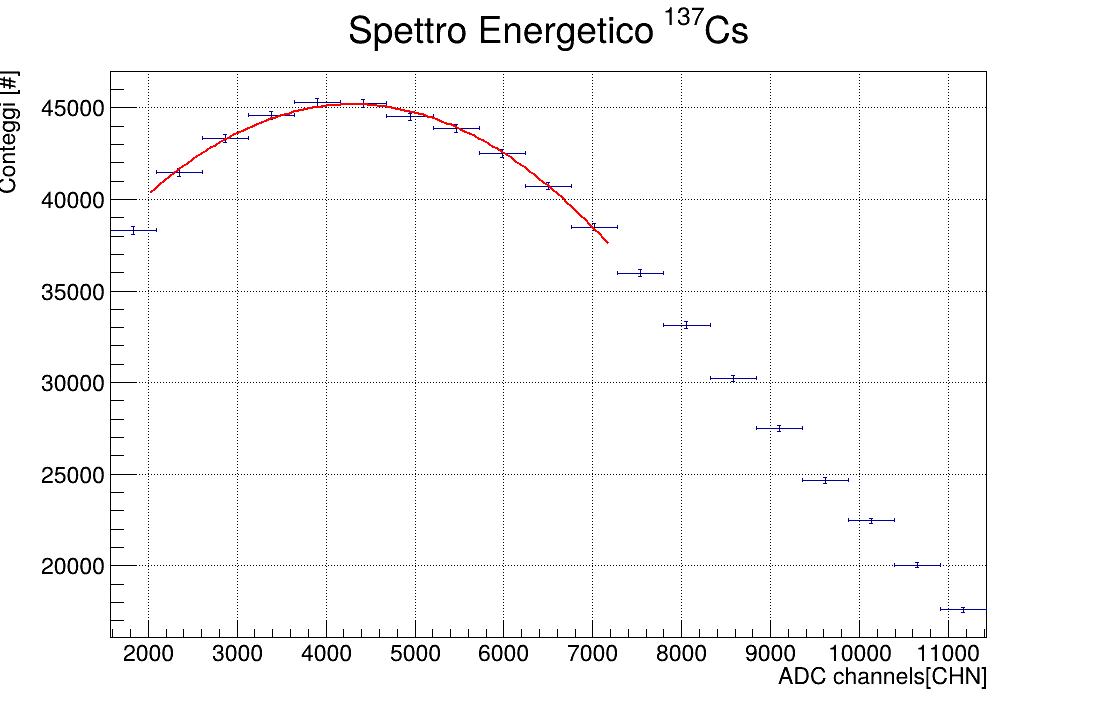
\includegraphics[width=0.65\linewidth]{fig2/cs137_Tmax.png}
    \caption{ \footnotesize Istogramma di conteggi per numero di canale del ${}^{137}$Cs (con accorpamento di \textit{bin}), con fit parabolico $y=ax^2+bx+c$ con parametri restituiti
    $a=(-9.2\pm0.3)$CHN$^{-2}$,
    $b=(7.9\pm0.3)\text{CHN}^{-1}$,
    $c=(2.81\pm0.07)\cdot10^5$, $\chi^2 = 5.8$ e d.o.f.$=7$.
    }
    \label{fig:cs_tmax}
\end{figure}
\newpage
Questa stima \textit{non} risulta statisticamente compatibile con il valore atteso (Z-score$=2.26$)
$$T_\text{max,Cs,att} = (153.6\pm0.3)\text{keV}$$
Questo è probabilmente dovuto in primo luogo al fatto che l'incertezza associata al massimo deriva da quelle sui parametri dei fit (e risulta quindi sottostimata), in secondo luogo al fatto che intorno al massimo, come si vedrà nella sezione successiva, l'andamento dell'istogramma è la sovrapposizione di diversi massimi locali che è stato necessario accorpare per poter determinare un solo massimo globale: questo ha probablimente influito nel peggiorare la stima di $T_\text{max,Cs}$

\subsubsection{Verifica della risoluzione attesa $\mathbf{R_{att}}$}
Si vuole ora stimare la risoluzione sperimentale dell'apparato; a tal fine si è acquisito uno spettro con zoom a bassi canali. 

\begin{figure} [H]
    \centering
    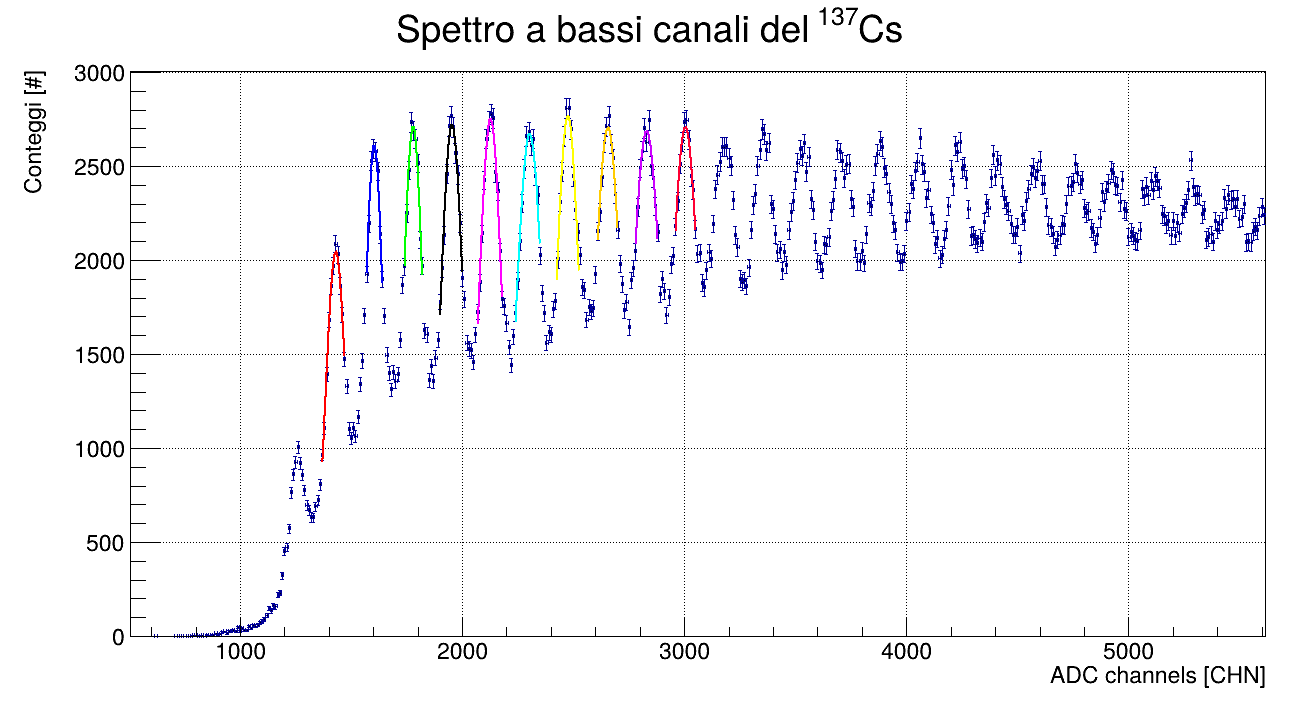
\includegraphics[width=0.82\linewidth]{fig2/fit_picchi.png}
    \caption{ \footnotesize Istogramma di conteggi per numero di canale per il ${}^{137}$Cs con zoom a bassi canali ($G_{ampl}=28$dB, $V_{bias}=54$V).}
    \label{fig:cesio-zoom1}
\end{figure}

Dal grafico \ref{fig:cesio-zoom1} si osservano i singoli picchi delle celle del SiPM accese, per ciascuno dei quali è stato effettuato un fit gaussiano da cui si sono estratti i valori medi $p_i$ e le rispettive deviazioni standard $\sigma_{p,i}$. Si possono allora calcolare diverse stime $\Delta_{pp, i}$ (vedi Tabella \ref{tab:zoomcs}) tra picchi consecutivi e dopo aver dimostrato che queste appartengono alla stessa popolazione tramite il test di Gauss, si calcolano la media pesata $\langle\Delta_{pp}\rangle$ e la sua incertezza $\sigma_{pp}$, ottenendo $$ \langle\Delta_{pp}\rangle= ( 1.7  \pm  0.3  )\cdot10^{2}\text{ CHN} $$

Si è verificato infine che la risoluzione attesa dalle caratteristiche dello strumento $$R_{att}=\sqrt{ \frac{\langle\Delta_{pp}\rangle}{\langle CHN\rangle_{ci}} \cdot \left( 1 + \left(\frac{\sigma_{pp}}{\langle\Delta_{pp}\rangle} \right)^2 \right)} =  0.095 \pm  0.009  $$ 
è statisticamente compatibile con quella sperimentale $R_{exp}$ (\ref{eq:R_exp}).








